\documentclass[a4paper]{article}

% content/resources/templates/preamble.tex
\usepackage[margin=0.6in]{geometry}
\author{Milav Dabgar}
\usepackage{amsmath,amssymb,amsthm}
\usepackage{booktabs}
\usepackage{multirow}
\usepackage{xcolor}
\usepackage{tcolorbox}
\tcbuselibrary{breakable,skins}
\usepackage[colorlinks=true,linkcolor=blue]{hyperref}
\usepackage{titlesec}
\usepackage{enumitem}
\usepackage{tikz}
\usepackage{pgfplots}
\usepackage{circuitikz}
\usepackage[version=4]{mhchem}
\usepackage{longtable}
\usepackage{array}
\usepackage{float}
\usepackage{caption}
\usepackage{listings}

\lstset{
  basicstyle=\small\ttfamily,
  breaklines=true,
  breakatwhitespace=false,
  postbreak=\mbox{\textcolor{red}{$\hookrightarrow$}\space},
  float=false,
  numbers=left,
  numberstyle=\tiny\color{gray},
  numbersep=10pt,
  xleftmargin=2em,
  keywordstyle=\color{blue},
  commentstyle=\color{green!60!black},
  stringstyle=\color{purple},
  backgroundcolor=\color{gray!5},
  showstringspaces=false,
  tabsize=2,
  captionpos=b,
  keepspaces=true,
  columns=flexible
}

\pgfplotsset{compat=1.18}
\usetikzlibrary{shapes,arrows,positioning,calc,patterns,decorations.pathmorphing,decorations.markings,arrows.meta}

% Color scheme
\definecolor{headcolor}{RGB}{0,102,204}
\definecolor{keycolor}{RGB}{220,20,60}
\definecolor{solutioncolor}{RGB}{34,139,34}
\definecolor{mnemoniccolor}{RGB}{148,0,211}
\definecolor{codecolor}{RGB}{0,0,100}

% Spacing
\setlength{\parskip}{3pt}
\setlist[itemize]{nosep}
\setlist[enumerate]{nosep}

% Title formatting
\titleformat{\section}{\Large\bfseries\color{headcolor}}{\thesection}{1em}{}
\titleformat{\subsection}{\large\bfseries\color{headcolor}}{\thesubsection}{1em}{}

% Pandoc tightlist compatibility
\providecommand{\tightlist}{%
  \setlength{\itemsep}{0pt}\setlength{\parskip}{0pt}}

% Pandoc longtable compatibility
\newcounter{none}
\def\thenone{}


% Custom commands for GTU solutions
% This file defines semantic commands for consistent formatting

% Question command with automatic formatting
\newcommand{\question}[2]{%
  \section*{Question #1}%
  \textbf{#2}%
}

% OR question variant
\newcommand{\questionor}[2]{%
  \section*{Question #1 OR}%
  \textbf{#2}%
}

% Proper table environment with caption
\newenvironment{answertable}[1]{%
  \begin{table}[htbp]
  \centering
  \caption{#1}
}{%
  \end{table}
}

% Proper figure environment for diagrams
\newenvironment{answerdiagram}[1]{%
  \begin{figure}[htbp]
  \centering
  \caption{#1}
}{%
  \end{figure}
}

% Semantic markup for key terms
\newcommand{\keyword}[1]{\textbf{#1}}
\newcommand{\code}[1]{\texttt{#1}}
\newcommand{\classname}[1]{\texttt{#1}}
\newcommand{\methodname}[1]{\texttt{#1}}

% Proper quotation marks
\newcommand{\mnemonic}[1]{``#1''}


% content/resources/templates/english-boxes.tex
% This file is currently empty - it exists to maintain consistency with the import structure.
% Add custom environments here if needed in the future.


% Redefine environments to avoid float-in-box errors
\renewenvironment{answertable}[1]{%
  \begin{center}
  \captionof{table}{#1}
}{%
  \end{center}
}

\renewenvironment{answerdiagram}[1]{%
  \begin{center}
  \captionof{figure}{#1}
}{%
  \end{center}
}

\title{Embedded System (4343204) - Winter 2024 Solution}
\date{December 03, 2024}

\begin{document}
\maketitle

% Define missing style locally if needed
\tikzset{
  gtu decision/.style={diamond, aspect=1.5, draw, fill=blue!10, align=center, font=\small}
}

\questionmarks{1(a)}{3}{Write the size of RAM, Flash and EEPROM memory in ATmega32 and explain its need in microcontroller.}

\begin{solutionbox}
\textbf{ATmega32 memory specifications and their importance in microcontroller operation:}

\begin{answertable}{Memory Sizes in ATmega32}
\begin{tabulary}{\linewidth}{|L|L|L|}
\hline
\textbf{Memory Type} & \textbf{Size} & \textbf{Purpose} \\ \hline
SRAM (RAM) & 2 KB & Variables and stack storage \\ \hline
Flash & 32 KB & Program storage \\ \hline
EEPROM & 1 KB & Non-volatile data storage \\ \hline
\end{tabulary}
\end{answertable}

\begin{itemize}
    \item \keyword{RAM}: Temporary storage for variables during program execution
    \item \keyword{Flash}: Permanent storage for program instructions and constants
    \item \keyword{EEPROM}: Long-term storage for data that must survive power cycles
\end{itemize}
\end{solutionbox}

\begin{mnemonicbox}
\mnemonic{RAM for Run, Flash for Function, EEPROM for Eternity}
\end{mnemonicbox}

\questionmarks{1(b)}{4}{Discuss RAM memory of ATmega32.}

\begin{solutionbox}
\textbf{ATmega32's RAM (SRAM) is organized into different sections for specific purposes.}

\begin{answerdiagram}{ATmega32 RAM Organization}
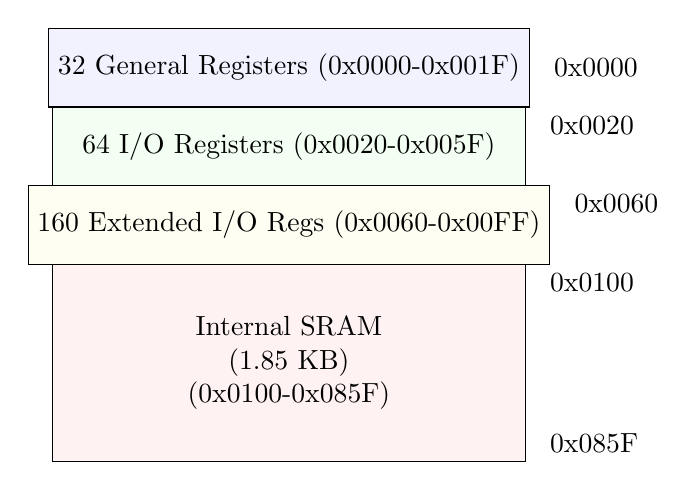
\begin{tikzpicture}[node distance=0cm, outer sep=0pt]
    \node [draw, rectangle, minimum width=6cm, minimum height=1cm, fill=blue!5] (regs) {32 General Registers (0x0000-0x001F)};
    \node [draw, rectangle, minimum width=6cm, minimum height=1cm, fill=green!5, below=of regs] (io) {64 I/O Registers (0x0020-0x005F)};
    \node [draw, rectangle, minimum width=6cm, minimum height=1cm, fill=yellow!5, below=of io] (ext) {160 Extended I/O Regs (0x0060-0x00FF)};
    \node [draw, rectangle, minimum width=6cm, minimum height=2.5cm, fill=red!5, below=of ext, align=center] (sram) {Internal SRAM\\(1.85 KB)\\(0x0100-0x085F)};
    
    \node [right=0.2cm of regs] {0x0000};
    \node [right=0.2cm of io.north east, anchor=north west] {0x0020};
    \node [right=0.2cm of ext.north east, anchor=north west] {0x0060};
    \node [right=0.2cm of sram.north east, anchor=north west] {0x0100};
    \node [right=0.2cm of sram.south east, anchor=south west] {0x085F};
\end{tikzpicture}
\end{answerdiagram}

\begin{itemize}
    \item \keyword{Register File}: First 32 locations (0x0000-0x001F)
    \item \keyword{I/O Registers}: Standard I/O space (0x0020-0x005F)
    \item \keyword{Extended I/O}: Additional peripheral registers (0x0060-0x00FF)
    \item \keyword{Data Memory}: General purpose SRAM (0x0100-0x085F)
\end{itemize}
\end{solutionbox}

\begin{mnemonicbox}
\mnemonic{Registers, I/O, Extended, Data - RAM's Efficient Design}
\end{mnemonicbox}

\questionmarks{1(c)}{7}{Define Real Time Operating System and Explain Characteristics of it.}

\begin{solutionbox}
\textbf{A Real-Time Operating System (RTOS) is a specialized operating system designed to process data and events with precise timing constraints.}

\begin{answertable}{Key Characteristics of RTOS}
\begin{tabulary}{\linewidth}{|L|L|}
\hline
\textbf{Characteristic} & \textbf{Description} \\ \hline
Determinism & Guaranteed response times for tasks \\ \hline
Preemptive Scheduling & Higher priority tasks can interrupt lower ones \\ \hline
Low Latency & Minimal delay between event and response \\ \hline
Priority-Based & Tasks are assigned priorities for execution \\ \hline
Task Management & Provides mechanisms for task creation, deletion, and synchronization \\ \hline
Resource Management & Prevents resource conflicts and deadlocks \\ \hline
Reliability & Robust operation even under peak loads \\ \hline
\end{tabulary}
\end{answertable}

\begin{itemize}
    \item \keyword{Multitasking}: Supports concurrent execution of multiple tasks
    \item \keyword{Small Footprint}: Optimized for embedded systems with limited resources
    \item \keyword{Time Management}: Precise timing services with microsecond resolution
    \item \keyword{Kernel Services}: IPC, mutex, semaphores for task coordination
\end{itemize}
\end{solutionbox}

\begin{mnemonicbox}
\mnemonic{Deterministic Preemptive Tasks Run On Strict Timelines}
\end{mnemonicbox}

\questionmarks{1(c OR)}{7}{What is Embedded System? Draw and Explain General block diagram of Embedded system.}

\begin{solutionbox}
\textbf{An Embedded System is a dedicated computer system designed to perform specific functions within a larger mechanical or electrical system, often with real-time constraints.}

\begin{answerdiagram}{General Block Diagram of Embedded System}
\begin{tikzpicture}[node distance=1.5cm, auto, >=latex, thick]
    % Central Unit
    \node [gtu block, minimum width=3cm, minimum height=1.5cm] (cpu) {Processing Unit\\(Cpu/Microcontroller)};
    
    % Peripherals in a cross pattern
    \node [gtu block, left=of cpu] (input) {Input Devices};
    \node [gtu block, right=of cpu] (output) {Output Devices};
    \node [gtu block, above=of cpu] (psu) {Power Supply};
    \node [gtu block, below=of cpu] (comm) {Communication\\Interface};
    
    % Memory and others
    \node [gtu block, above right=of cpu] (mem) {Memory\\(RAM/ROM)};
    \node [gtu block, below left=of cpu] (sensors) {Sensors};
    \node [gtu block, below right=of cpu] (store) {Storage};

    % Connections
    \draw [->] (psu) -- (cpu);
    \draw [->] (input) -- (cpu);
    \draw [->] (cpu) -- (output);
    \draw [<->] (cpu) -- (comm);
    \draw [<->] (cpu) -- (mem);
    \draw [->] (sensors) -- (input); % Logical flow: Sensor -> Input -> CPU
    \draw [<->] (cpu) -- (store);
    
    % Power distribution lines (implied or simplified)
    \draw [dashed, ->] (psu) -| (input);
    \draw [dashed, ->] (psu) -| (output);
\end{tikzpicture}
\end{answerdiagram}

\begin{answertable}{Embedded System Components}
\begin{tabulary}{\linewidth}{|L|L|}
\hline
\textbf{Component} & \textbf{Function} \\ \hline
Processing Unit & Executes program instructions (microcontroller/microprocessor) \\ \hline
Memory & Stores program and data (RAM, ROM, Flash) \\ \hline
Input/Output & Interfaces with external devices \\ \hline
Communication & Connects to other systems or networks \\ \hline
Power Supply & Provides regulated power \\ \hline
Sensors & Gather environmental data \\ \hline
\end{tabulary}
\end{answertable}

\begin{itemize}
    \item \keyword{Application-Specific}: Designed for dedicated tasks
    \item \keyword{Resource-Constrained}: Limited processing power and memory
    \item \keyword{Real-Time}: Responds to events within timing constraints
    \item \keyword{High Reliability}: Must operate continuously without failure
\end{itemize}
\end{solutionbox}


\questionmarks{2(a)}{3}{Write different Criteria for choosing microcontroller for any application design in embedded system.}

\begin{solutionbox}
\textbf{Selecting the right microcontroller requires evaluating multiple criteria based on application requirements.}

\begin{answertable}{Microcontroller Selection Criteria}
\begin{tabulary}{\linewidth}{|L|L|}
\hline
\textbf{Criterion} & \textbf{Considerations} \\ \hline
Performance & CPU speed, MIPS, bit width (8/16/32) \\ \hline
Memory & Flash, RAM, EEPROM capacity \\ \hline
Power Consumption & Operating voltage, sleep modes \\ \hline
I/O Capabilities & Number of ports, special functions \\ \hline
Peripherals & ADC, timers, communication interfaces \\ \hline
Cost & Unit price, development tools \\ \hline
Form Factor & Size, package type, pin count \\ \hline
\end{tabulary}
\end{answertable}

\begin{itemize}
    \item \keyword{Application Requirements}: Specific features needed for the application
    \item \keyword{Development Environment}: Available compilers, debuggers, libraries
    \item \keyword{Future Expansion}: Scalability for future enhancements
\end{itemize}
\end{solutionbox}

\begin{mnemonicbox}
\mnemonic{Performance Memory Power I/O Cost}
\end{mnemonicbox}

\questionmarks{2(b)}{4}{Draw and Explain TCCR0 register.}

\begin{solutionbox}
\textbf{Timer/Counter Control Register 0 (TCCR0) controls the operation of Timer/Counter0 in ATmega32.}

\begin{answerdiagram}{TCCR0 Register}
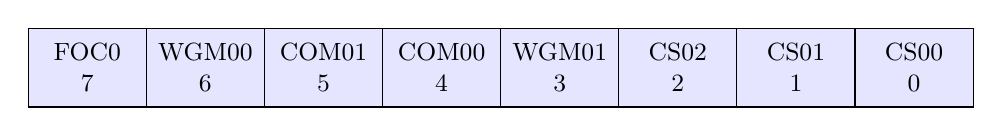
\begin{tikzpicture}[
    node distance=0cm,
    outer sep=0pt,
    bit/.style={draw, rectangle, minimum width=1.5cm, minimum height=1cm, align=center, font=\small}
]
    \node [bit, fill=blue!10] (b7) {FOC0\\7};
    \node [bit, fill=blue!10, right=of b7] (b6) {WGM00\\6};
    \node [bit, fill=blue!10, right=of b6] (b5) {COM01\\5};
    \node [bit, fill=blue!10, right=of b5] (b4) {COM00\\4};
    \node [bit, fill=blue!10, right=of b4] (b3) {WGM01\\3};
    \node [bit, fill=blue!10, right=of b3] (b2) {CS02\\2};
    \node [bit, fill=blue!10, right=of b2] (b1) {CS01\\1};
    \node [bit, fill=blue!10, right=of b1] (b0) {CS00\\0};
\end{tikzpicture}
\end{answerdiagram}

\begin{answertable}{TCCR0 Bit Functions}
\begin{tabulary}{\linewidth}{|L|L|L|}
\hline
\textbf{Bits} & \textbf{Name} & \textbf{Function} \\ \hline
7 & FOC0 & Force Output Compare \\ \hline
6,3 & WGM01:0 & Waveform Generation Mode \\ \hline
5,4 & COM01:0 & Compare Match Output Mode \\ \hline
2,1,0 & CS02:0 & Clock Select (Prescaler) \\ \hline
\end{tabulary}
\end{answertable}

\begin{itemize}
    \item \keyword{WGM01:0}: Determines timer operating mode (Normal, CTC, PWM)
    \item \keyword{COM01:0}: Controls OC0 pin output behavior
    \item \keyword{CS02:0}: Selects clock source and prescaler value
\end{itemize}
\end{solutionbox}

\begin{mnemonicbox}
\mnemonic{Force Waveform Compare Clock Select}
\end{mnemonicbox}

\questionmarks{2(c)}{7}{List timers of ATmega32 and Explain working modes of any one timer in detail.}

\begin{solutionbox}
\textbf{ATmega32 features multiple timers with various capabilities and operating modes.}

\begin{answertable}{Timers in ATmega32}
\begin{tabulary}{\linewidth}{|L|L|L|L|}
\hline
\textbf{Timer} & \textbf{Type} & \textbf{Size} & \textbf{Features} \\ \hline
Timer0 & General Purpose & 8-bit & Simple timing, PWM \\ \hline
Timer1 & Advanced & 16-bit & Input capture, dual PWM \\ \hline
Timer2 & General Purpose & 8-bit & Asynchronous operation \\ \hline
\end{tabulary}
\end{answertable}

\textbf{Timer0 Working Modes:}
\begin{itemize}
    \item \textbf{Normal Mode}:
    \begin{itemize}
        \item Counter increments from 0 to 255 then overflows back to 0
        \item Overflow interrupt can be generated
        \item Used for simple timing and delay generation
    \end{itemize}
    
    \item \textbf{CTC (Clear Timer on Compare) Mode}:
    \begin{itemize}
        \item Counter resets when it reaches OCR0 value
        \item Allows precise frequency generation
        \item Compare match interrupt can be generated
    \end{itemize}
    
    \item \textbf{Fast PWM Mode}:
    \begin{itemize}
        \item Counter counts from 0 to 255
        \item Output toggles at overflow and compare match
        \item High frequency PWM generation
    \end{itemize}
    
    \item \textbf{Phase Correct PWM Mode}:
    \begin{itemize}
        \item Counter counts up then down (0$\to$255$\to$0)
        \item Symmetric PWM waveform generation
        \item Lower frequency but better resolution than Fast PWM
    \end{itemize}
\end{itemize}
\end{solutionbox}

\begin{mnemonicbox}
\mnemonic{Normal Compares Fast Phase - Timer Modes Matter}
\end{mnemonicbox}

\questionmarks{2(a OR)}{3}{List various embedded system applications. Explain any one in brief.}

\begin{solutionbox}
\textbf{Embedded systems are found in numerous applications across various domains.}

\begin{answertable}{Embedded System Applications}
\begin{tabulary}{\linewidth}{|L|L|}
\hline
\textbf{Domain} & \textbf{Applications} \\ \hline
Consumer & Smart appliances, entertainment systems \\ \hline
Automotive & Engine control, safety systems, infotainment \\ \hline
Industrial & Process control, automation, robotics \\ \hline
Medical & Patient monitoring, imaging, implantable devices \\ \hline
Communications & Routers, modems, network switches \\ \hline
Aerospace & Flight control, navigation, life support \\ \hline
\end{tabulary}
\end{answertable}

\textbf{Smart Home Automation System:}
A smart home system uses embedded controllers to monitor and control household devices. Sensors detect environmental conditions like temperature and motion, while microcontrollers process this data and control actuators such as HVAC systems, lighting, and security devices. The system can be programmed for autonomous operation or user control via smartphone apps, providing convenience, energy efficiency, and enhanced security.
\end{solutionbox}

\begin{mnemonicbox}
\mnemonic{Consumers Automate Industry Medical Communications Aerospace}
\end{mnemonicbox}

\questionmarks{2(b OR)}{4}{Explain the function of DDRA, PINA and PORTA registers in ATmega32 microcontroller.}

\begin{solutionbox}
\textbf{The three registers control the operation of Port A in ATmega32, each serving a distinct purpose.}

\begin{answertable}{Port A Registers}
\begin{tabulary}{\linewidth}{|L|L|L|}
\hline
\textbf{Register} & \textbf{Function} & \textbf{Operation} \\ \hline
DDRA & Data Direction & Configures pins as input (0) or output (1) \\ \hline
PORTA & Data Register & Sets output values or enables pull-ups \\ \hline
PINA & Port Input Pins & Reads actual pin states \\ \hline
\end{tabulary}
\end{answertable}

\textbf{Example Configurations:}
\begin{codebox}
\begin{lstlisting}[language=C]
DDRA = 0xFF;  // All pins as output
PORTA = 0xA5; // Set alternating pattern (10100101)

DDRA = 0x00;  // All pins as input
PORTA = 0xFF; // Enable internal pull-ups on all pins
data = PINA;  // Read current pin states
\end{lstlisting}
\end{codebox}

\begin{itemize}
    \item \keyword{Bit-Level Control}: Each bit controls corresponding pin
    \item \keyword{Atomic Operations}: Individual bits can be modified
    \item \keyword{Read-Modify-Write}: Common operation pattern
\end{itemize}
\end{solutionbox}

\begin{mnemonicbox}
\mnemonic{Direction Determines, Port Provides, PIN Perceives}
\end{mnemonicbox}

\questionmarks{2(c OR)}{7}{Draw Status Register of ATmega32 and explain it in detail.}

\begin{solutionbox}
\textbf{The Status Register (SREG) in ATmega32 contains processor status flags affected by arithmetic operations and controls interrupts.}

\begin{answerdiagram}{Status Register (SREG)}
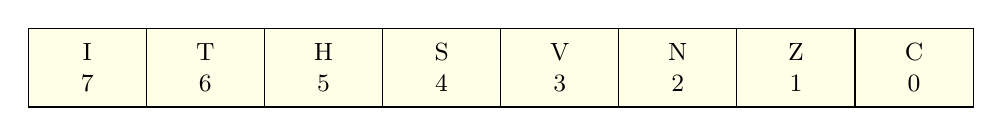
\begin{tikzpicture}[
    node distance=0cm,
    outer sep=0pt,
    bit/.style={draw, rectangle, minimum width=1.5cm, minimum height=1cm, align=center, font=\small}
]
    \node [bit, fill=yellow!10] (b7) {I\\7};
    \node [bit, fill=yellow!10, right=of b7] (b6) {T\\6};
    \node [bit, fill=yellow!10, right=of b6] (b5) {H\\5};
    \node [bit, fill=yellow!10, right=of b6] (b5) {H\\5}; % Fix duplication if any, wait, just typing carefully
    \node [bit, fill=yellow!10, right=of b6] (b5) {H\\5};
    % Re-doing nodes correctly
    \node [bit, fill=yellow!10, right=of b6] (b5node) {H\\5};
    \node [bit, fill=yellow!10, right=of b5node] (b4) {S\\4};
    \node [bit, fill=yellow!10, right=of b4] (b3) {V\\3};
    \node [bit, fill=yellow!10, right=of b3] (b2) {N\\2};
    \node [bit, fill=yellow!10, right=of b2] (b1) {Z\\1};
    \node [bit, fill=yellow!10, right=of b1] (b0) {C\\0};
\end{tikzpicture}
\end{answerdiagram}

\begin{answertable}{SREG Bit Functions}
\begin{tabulary}{\linewidth}{|L|L|L|L|}
\hline
\textbf{Bit} & \textbf{Name} & \textbf{Function} & \textbf{Set When} \\ \hline
7 & I & Global Interrupt Enable & Programmatically enabled \\ \hline
6 & T & Bit Copy Storage & Used for bit copy instructions \\ \hline
5 & H & Half Carry Flag & Half-carry in BCD operations \\ \hline
4 & S & Sign Flag & N$\oplus$V (used for signed operations) \\ \hline
3 & V & Two's Complement Overflow & Arithmetic overflow occurs \\ \hline
2 & N & Negative Flag & Result is negative (MSB=1) \\ \hline
1 & Z & Zero Flag & Result is zero \\ \hline
0 & C & Carry Flag & Carry occurs in arithmetic \\ \hline
\end{tabulary}
\end{answertable}

\begin{itemize}
    \item \keyword{Arithmetic Feedback}: Indicates result status
    \item \keyword{Conditional Branches}: Used by branch instructions
    \item \keyword{Interrupt Control}: I-bit enables/disables all interrupts
    \item \keyword{Access Methods}: Directly addressable via IN/OUT instructions
\end{itemize}
\end{solutionbox}


% Question 3
\questionmarks{3(a)}{3}{Write a short note on Harvard Architecture of AVR microcontroller.}

\begin{solutionbox}
\textbf{Harvard Architecture is a fundamental design principle of AVR microcontrollers, separating program and data memory.}

\begin{answerdiagram}{Harvard Architecture}
\begin{tikzpicture}[node distance=2cm, auto, >=latex, thick]
    \node [gtu block, minimum height=1.5cm] (cpu) {CPU Core};
    \node [gtu block, align=center, above right=1cm and 0.5cm of cpu] (pm) {Program Memory\\(Flash)};
    \node [gtu block, align=center, below right=1cm and 0.5cm of cpu] (dm) {Data Memory\\(SRAM)};
    
    \draw [->] (cpu) -- node[sloped, above] {Instruction Bus} (pm);
    \draw [->] (cpu) -- node[sloped, above] {Data Bus} (dm);
    % Actually Harvard has separate buses for fetch and data access.
    % Usually depicted as CPU accessing both independently.
    % Let's refine based on typical diagrams:
    % CPU <==> Flash
    % CPU <==> SRAM
\end{tikzpicture}
% Refining the diagram to be more consistent with standard representations
\begin{tikzpicture}[node distance=2cm, auto, >=latex, thick]
    \node [gtu block] (cpu) {CPU Core};
    \node [gtu block, right=3cm of cpu] (periph) {Peripherals}; % Optional context
    \node [gtu block, above=1cm of cpu] (flash) {Program Memory\\(Flash)};
    \node [gtu block, below=1cm of cpu] (sram) {Data Memory\\(SRAM)};
    
    % Buses
    \draw [<->, double] (cpu) -- node[right] {Instruction Bus} (flash);
    \draw [<->, double] (cpu) -- node[right] {Data Bus} (sram);
\end{tikzpicture}
\end{answerdiagram}

\begin{itemize}
    \item \keyword{Separate Buses}: Independent buses for program and data memory
    \item \keyword{Parallel Access}: Can fetch instructions and access data simultaneously
    \item \keyword{Performance}: Increases execution speed by eliminating memory bottlenecks
    \item \keyword{Different Widths}: Program memory is organized in 16-bit words, data memory in 8-bit bytes
\end{itemize}
\end{solutionbox}

\begin{mnemonicbox}
\mnemonic{Program and Data Paths Are Separate}
\end{mnemonicbox}

\questionmarks{3(b)}{4}{List Registers associated with Serial Communication (RS232) and explain steps to interface it with ATmega32.}

\begin{solutionbox}
\textbf{ATmega32 uses USART (Universal Synchronous Asynchronous Receiver Transmitter) for serial communication.}

\begin{answertable}{USART Registers}
\begin{tabulary}{\linewidth}{|L|L|}
\hline
\textbf{Register} & \textbf{Function} \\ \hline
UDR & USART Data Register (transmit/receive) \\ \hline
UCSRA & USART Control and Status Register A \\ \hline
UCSRB & USART Control and Status Register B \\ \hline
UCSRC & USART Control and Status Register C \\ \hline
UBRRH/UBRRL & USART Baud Rate Registers \\ \hline
\end{tabulary}
\end{answertable}

\textbf{Steps to Interface RS232:}
\begin{enumerate}
    \item \textbf{Hardware Connection}:
    \begin{itemize}
        \item Connect ATmega32's TXD (PD1) and RXD (PD0) to MAX232
        \item Connect MAX232 to RS232 port or connector
    \end{itemize}
    \item \textbf{Initialize USART}:
    \begin{itemize}
        \item Set baud rate (UBRR)
        \item Set frame format (data bits, parity, stop bits)
        \item Enable transmitter and/or receiver
    \end{itemize}
    \item \textbf{Data Transmission/Reception}:
    \begin{itemize}
        \item Check status flags before operation
        \item Write to UDR to transmit
        \item Read from UDR to receive
    \end{itemize}
\end{enumerate}
\end{solutionbox}

\begin{mnemonicbox}
\mnemonic{Connect, Configure Baud, Enable, Transmit/Receive}
\end{mnemonicbox}

\questionmarks{3(c)}{7}{Explain Bit-wise logical operations in AVR C programming with necessary examples.}

\begin{solutionbox}
\textbf{Bit-wise operations manipulate individual bits in a byte or word, essential for embedded programming.}

\begin{answertable}{Bit-wise Operators in AVR C}
\begin{tabulary}{\linewidth}{|C|L|L|L|}
\hline
\textbf{Operator} & \textbf{Operation} & \textbf{Example} & \textbf{Result} \\ \hline
\& & AND & 0xA5 \& 0x0F & 0x05 \\ \hline
\textbar & OR & 0x50 \textbar{} 0x0F & 0x5F \\ \hline
\textasciicircum & XOR & 0x55 \textasciicircum{} 0xFF & 0xAA \\ \hline
\textasciitilde & NOT & \textasciitilde{}0x55 & 0xAA \\ \hline
\textless{}\textless & Left Shift & 0x01 \textless{}\textless{} 3 & 0x08 \\ \hline
\textgreater{}\textgreater & Right Shift & 0x80 \textgreater{}\textgreater{} 3 & 0x10 \\ \hline
\end{tabulary}
\end{answertable}

\textbf{Example: Setting and Clearing Bits}
\begin{codebox}
\begin{lstlisting}[language=C]
// Set bit 3 of PORTB
PORTB |= (1 << 3);   // PORTB = PORTB | 0b00001000

// Clear bit 5 of PORTB
PORTB &= ~(1 << 5);  // PORTB = PORTB & 0b11011111

// Toggle bit 2 of PORTB
PORTB ^= (1 << 2);   // PORTB = PORTB ^ 0b00000100

// Check if bit 4 is set
if (PINB & (1 << 4)) {
    // Bit 4 is set
}
\end{lstlisting}
\end{codebox}
\end{solutionbox}

\begin{mnemonicbox}
\mnemonic{AND clears, OR sets, XOR toggles, Shift multiplies/divides}
\end{mnemonicbox}

\questionmarks{3(a OR)}{3}{Explain RESET circuit for the ATmega32 microcontroller.}

\begin{solutionbox}
\textbf{The reset circuit ensures proper initialization of ATmega32 when power is applied or during system reset.}

\begin{answerdiagram}{Reset Circuit}
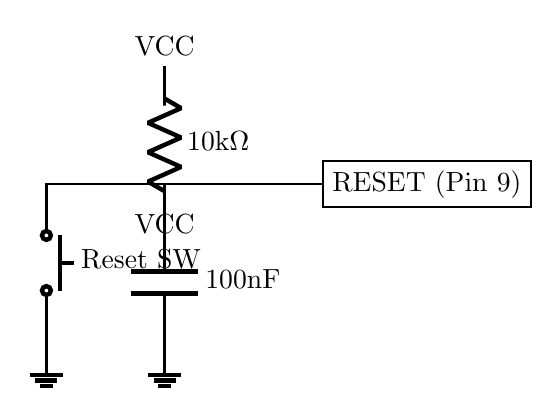
\begin{tikzpicture}[auto, >=latex, thick]
    % Components
    \node (vcc) {VCC};
    \node [below=0.5cm of vcc] (res) {}; % Placeholder or implicit
    % Actually let's use standard circuitikz logic or drawing
    \coordinate (top) at (0,2);
    \coordinate (bottom) at (0,-1);
    \coordinate (reset_pin) at (2,0.5);
    
    % Drawing simplified resistor/cap/switch structure
    \draw (0,2) node[above]{VCC} -- (0,1.5) to[R, l=10k$\Omega$] (0,0.5) -- (0,0);
    \draw (0,0.5) -- (2,0.5) node[right, draw] {RESET (Pin 9)};
    \draw (0,0) to[C, l=100nF] (0,-1.5) node[ground]{};
    \draw (0,0.5) -- (-1.5, 0.5) to[push button, l=Reset SW] (-1.5, -1.5) node[ground]{};
\end{tikzpicture}
\end{answerdiagram}

\begin{itemize}
    \item \keyword{Active-Low RESET}: Held low to reset the microcontroller
    \item \keyword{External Reset}: Manual reset button connects RESET pin to ground
    \item \keyword{Power-on Reset}: Auto-reset when power is first applied
    \item \keyword{Brown-out Detection}: Reset when voltage drops below threshold
    \item \keyword{Watchdog Timer}: Reset on software malfunction
\end{itemize}
\end{solutionbox}

\begin{mnemonicbox}
\mnemonic{Pull Up, Push Button, Power Starts, Voltage Drops}
\end{mnemonicbox}

\questionmarks{3(b OR)}{4}{List Registers associated with EEPROM and write steps to interface EEPROM of ATmega32.}

\begin{solutionbox}
\textbf{ATmega32 has on-chip EEPROM with dedicated registers for access control.}

\begin{answertable}{EEPROM Registers}
\begin{tabulary}{\linewidth}{|L|L|}
\hline
\textbf{Register} & \textbf{Function} \\ \hline
EEARH/EEARL & EEPROM Address Registers \\ \hline
EEDR & EEPROM Data Register \\ \hline
EECR & EEPROM Control Register \\ \hline
\end{tabulary}
\end{answertable}

\textbf{Steps to Interface EEPROM:}
\begin{enumerate}
    \item \textbf{Wait for Completion}: Check if previous write operation is complete (EEWE bit in EECR)
    \item \textbf{Set Address}: Load address into EEARH:EEARL (16-bit address)
    \item \textbf{Read or Write Operation}:
    \begin{itemize}
        \item For read: Set EERE bit in EECR, then read EEDR
        \item For write: Write data to EEDR, then set EEMWE and EEWE bits in EECR
    \end{itemize}
    \item \textbf{Wait for Completion}: Poll EEWE bit until it becomes zero
\end{enumerate}
\end{solutionbox}

\begin{mnemonicbox}
\mnemonic{Wait, Address, Data, Control, Wait}
\end{mnemonicbox}

\questionmarks{3(c OR)}{7}{Write a C program to generate square wave of 1KHz on the PORTC.2 pin continuously. Use Timer0, Normal mode, and 1:8 pre-scaler to create the delay. Assume XTAL = 8 MHz.}

\begin{solutionbox}
\textbf{Code Implementation:}

\begin{codebox}
\begin{lstlisting}[language=C]
#include <avr/io.h>

int main(void)
{
    // Configure PORTC.2 as output
    DDRC |= (1 << 2);  // Set PC2 as output
    
    // Timer0 configuration - Normal mode, 1:8 prescaler
    TCCR0 = (0 << WGM01) | (0 << WGM00) | (0 << CS02) | (1 << CS01) | (0 << CS00);
    
    // Calculate timer value for 1KHz (500us period, 250us half-period)
    // 8MHz/8 = 1MHz timer clock, 250 cycles for 250us
    // 256-250 = 6 (starting value for 250us)
    
    while (1)
    {
        // Toggle PORTC.2
        PORTC ^= (1 << 2);
        
        // Reset timer
        TCNT0 = 6;
        
        // Wait until timer overflows
        while (!(TIFR & (1 << TOV0)));
        
        // Clear overflow flag
        TIFR |= (1 << TOV0);
    }
    
    return 0;
}
\end{lstlisting}
\end{codebox}

\begin{itemize}
    \item \keyword{Frequency Calculation}: 1KHz = 1000Hz = 1ms period = 500$\mu$s half-period
    \item \keyword{Timer Clock}: 8MHz $\div$ 8 = 1MHz = 1$\mu$s per tick
    \item \keyword{Timer Ticks}: 250$\mu$s $\div$ 1$\mu$s = 250 ticks
    \item \keyword{Initial Value}: 256 - 250 = 6 (for overflow after 250 ticks)
\end{itemize}
\end{solutionbox}


% Question 4
\questionmarks{4(a)}{3}{Draw and Explain SPI based device interfacing diagram with ATmega32.}

\begin{solutionbox}
\textbf{SPI (Serial Peripheral Interface) is a synchronous serial communication protocol used to interface ATmega32 with peripheral devices.}

\begin{answerdiagram}{SPI Interfacing}
\begin{tikzpicture}[node distance=2.5cm, auto, >=latex, thick]
    \node [gtu block, minimum width=3cm, minimum height=3cm] (master) {ATmega32\\(Master)};
    \node [gtu block, minimum width=3cm, minimum height=3cm, right=of master] (slave) {SPI Device\\(Slave)};
    
    % Pins
    \node [anchor=east] at ([yshift=1cm]master.east) (m_ss) {SS (PB4)};
    \node [anchor=east] at ([yshift=0.33cm]master.east) (m_mosi) {MOSI (PB5)};
    \node [anchor=east] at ([yshift=-0.33cm]master.east) (m_miso) {MISO (PB6)};
    \node [anchor=east] at ([yshift=-1cm]master.east) (m_sck) {SCK (PB7)};
    
    \node [anchor=west] at ([yshift=1cm]slave.west) (s_cs) {CS};
    \node [anchor=west] at ([yshift=0.33cm]slave.west) (s_sdi) {SDI};
    \node [anchor=west] at ([yshift=-0.33cm]slave.west) (s_sdo) {SDO};
    \node [anchor=west] at ([yshift=-1cm]slave.west) (s_sck) {SCK};
    
    % Connections
    \draw [->] (m_ss) -- (s_cs);
    \draw [->] (m_mosi) -- (s_sdi);
    \draw [<-] (m_miso) -- (s_sdo);
    \draw [->] (m_sck) -- (s_sck);
\end{tikzpicture}
\end{answerdiagram}

\begin{itemize}
    \item \keyword{MOSI (Master Out Slave In)}: Data from master to slave
    \item \keyword{MISO (Master In Slave Out)}: Data from slave to master
    \item \keyword{SCK (Serial Clock)}: Synchronization clock provided by master
    \item \keyword{SS (Slave Select)}: Active-low signal to select specific slave device
\end{itemize}
\end{solutionbox}

\begin{mnemonicbox}
\mnemonic{Master Outputs, Slave Inputs, Clock Keeps Synchronization}
\end{mnemonicbox}

\questionmarks{4(b)}{4}{Draw and explain interfacing of Relay using ULN2803 with ATmega32.}

\begin{solutionbox}
\textbf{ULN2803 is an array of Darlington transistor pairs used to drive high-current devices like relays from microcontroller pins.}

\begin{answerdiagram}{Relay Interfacing using ULN2803}
\begin{tikzpicture}[auto, >=latex, thick, node distance=2cm]
    % Components
    \node [gtu block] (mcu) {ATmega32};
    \node [gtu block, right=of mcu] (uln) {ULN2803};
    \node [right=of uln, draw, rectangle, minimum width=2cm, minimum height=1.5cm] (relay) {Relay};
    
    % Connections
    \draw [->] ([yshift=0.5cm]mcu.east) -- node[above] {PD0} ([yshift=0.5cm]uln.west) node[left, font=\tiny] {IN1};
    \draw [->] ([yshift=0.5cm]uln.east) node[right, font=\tiny] {OUT1} -- ([yshift=0.5cm]relay.west);
    
    % Relay details
    \draw ([yshift=0.5cm]relay.east) -- ++(0.5,0) node[right] {NO};
    \draw (relay.north) -- ++(0,0.5) node[above] {VCC (12V)};
    
    % ULN Common and GND
    \draw (uln.south) -- ++(0,-0.5) node[ground] {};
    \draw (uln.north) -- ++(0,0.5) node[above] {COM (12V)};
\end{tikzpicture}
\end{answerdiagram}

\begin{itemize}
    \item \keyword{Current Amplification}: ULN2803 can sink up to 500mA per channel
    \item \keyword{Voltage Isolation}: Built-in diodes protect against inductive kickback
    \item \keyword{Multiple Channels}: 8 Darlington pairs in one package
    \item \keyword{High Voltage Rating}: Can handle up to 50V at outputs
\end{itemize}
\end{solutionbox}

\begin{mnemonicbox}
\mnemonic{Low Current Controls High Current Loads}
\end{mnemonicbox}

\questionmarks{4(c)}{7}{Draw an interfacing diagram of LM35 connected on ADC0 (pin 40) of ATmega32 and write AVR C program to display digital result on Port B. (use ADC in 8-bit mode).}

\begin{solutionbox}
\textbf{LM35 is a precision temperature sensor that outputs an analog voltage proportional to temperature.}

\begin{answerdiagram}{LM35 Interfacing}
\begin{tikzpicture}[auto, >=latex, thick]
    % LM35 Sensor
    \node [draw, rectangle, minimum width=1.5cm, minimum height=2cm] (lm35) {LM35};
    \node [above=0.5cm of lm35] (vcc) {+5V};
    \node [below=0.5cm of lm35, ground] (gnd) {};
    
    \draw (vcc) -- (lm35.north);
    \draw (lm35.south) -- (gnd);
    
    % MCU
    \node [gtu block, right=3cm of lm35, minimum height=3cm] (mcu) {ATmega32};
    \draw [->] (lm35.east) -- node[above] {Vout} node[below] {10mV/$^\circ$C} (mcu.west) node[right, font=\tiny] {PA0 (ADC0)};
\end{tikzpicture}
\end{answerdiagram}

\textbf{C Program:}
\begin{codebox}
\begin{lstlisting}[language=C]
#include <avr/io.h>
#include <util/delay.h>

int main(void)
{
    // Configure PORTB as output for displaying result
    DDRB = 0xFF;
    
    // Configure ADC
    // REFS0=1: AVCC reference
    // ADLAR=1: Left adjust for 8-bit reading from ADCH
    // MUX=00000: ADC0
    ADMUX = (0 << REFS1) | (1 << REFS0) | (1 << ADLAR) | 
            (0 << MUX4) | (0 << MUX3) | (0 << MUX2) | (0 << MUX1) | (0 << MUX0);
    
    // Enable ADC and set prescaler to 128
    ADCSRA = (1 << ADEN) | (1 << ADPS2) | (1 << ADPS1) | (1 << ADPS0);
    
    while (1)
    {
        // Start conversion
        ADCSRA |= (1 << ADSC);
        
        // Wait for conversion to complete
        while (ADCSRA & (1 << ADSC));
        
        // Display result on PORTB (8-bit from ADCH)
        PORTB = ADCH;
        
        // Wait before next reading
        _delay_ms(500);
    }
    
    return 0;
}
\end{lstlisting}
\end{codebox}

\begin{itemize}
    \item \keyword{Temperature Calculation}: LM35 outputs 10mV/$^\circ$C
    \item \keyword{ADC Configuration}: Left-adjusted for easy 8-bit reading
    \item \keyword{Resolution}: Using 8-bit mode gives approximately 1$^\circ$C resolution with 5V reference
    \item \keyword{Range}: Can measure 0-255$^\circ$C range (limited by 8-bit register)
\end{itemize}
\end{solutionbox}

\begin{mnemonicbox}
\mnemonic{Connect, Configure, Convert, Capture, Display}
\end{mnemonicbox}

\questionmarks{4(a OR)}{3}{Write an AVR C program to continuous monitor PA0 pin of port A. If it is HIGH, send HIGH to PC0 pin of port C; otherwise, send LOW to PC0 pin of port C.}

\begin{solutionbox}
\textbf{Code Implementation:}

\begin{codebox}
\begin{lstlisting}[language=C]
#include <avr/io.h>

int main(void)
{
    // Configure PA0 as input
    DDRA &= ~(1 << PA0);
    
    // Enable pull-up resistor on PA0
    PORTA |= (1 << PA0);
    
    // Configure PC0 as output
    DDRC |= (1 << PC0);
    
    while (1)
    {
        // Check if PA0 is HIGH
        if (PINA & (1 << PA0))
        {
            // Set PC0 HIGH
            PORTC |= (1 << PC0);
        }
        else
        {
            // Set PC0 LOW
            PORTC &= ~(1 << PC0);
        }
    }
    
    return 0;
}
\end{lstlisting}
\end{codebox}

\begin{itemize}
    \item \keyword{Input Configuration}: Set as input with pull-up resistor
    \item \keyword{Continuous Monitoring}: Infinite loop checks pin state
    \item \keyword{Output Action}: PC0 mirrors PA0 state
    \item \keyword{Efficient Code}: Simple conditional statement for pin monitoring
\end{itemize}
\end{solutionbox}

\begin{mnemonicbox}
\mnemonic{Configure, Monitor, Mirror}
\end{mnemonicbox}

\questionmarks{4(b OR)}{4}{Draw ATmega32 pin diagram and write function of Vcc, AVcc and Aref pin.}

\begin{solutionbox}
\textbf{ATmega32 has 40 pins organized in a DIP package, with power supply pins having distinct functions.}

\begin{answerdiagram}{ATmega32 Pin Diagram}
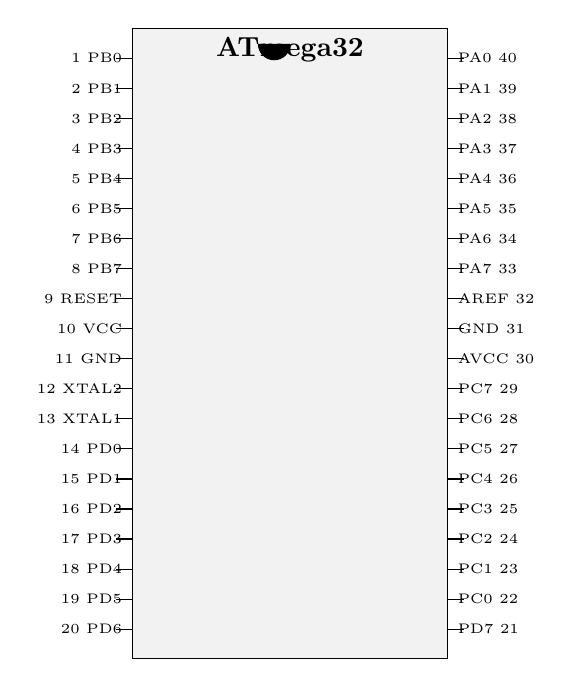
\begin{tikzpicture}[
    pin/.style={draw, rectangle, minimum width=0.8cm, minimum height=0.5cm, font=\tiny},
    ic/.style={draw, rectangle, minimum width=4cm, minimum height=8cm, fill=black!5}
]
    \node [ic] (atmega) {};
    \node [anchor=north, font=\bfseries] at (atmega.north) {ATmega32};
    \draw [fill=black] (atmega.north) ++(0,-0.2) arc (0:-180:0.2); % Notch
    
    % Left Pins (1-20)
    \foreach \i/\label in {1/PB0, 2/PB1, 3/PB2, 4/PB3, 5/PB4, 6/PB5, 7/PB6, 8/PB7, 9/RESET, 10/VCC, 11/GND, 12/XTAL2, 13/XTAL1, 14/PD0, 15/PD1, 16/PD2, 17/PD3, 18/PD4, 19/PD5, 20/PD6} {
         \node [left, font=\tiny] at ($(atmega.north west)!{\i/21}!(atmega.south west)$) {\i\ \label};
         \draw ($(atmega.north west)!{\i/21}!(atmega.south west)$) -- ++(-0.2,0);
    }
    
    % Right Pins (40-21)
    \foreach \i/\label in {1/PA0, 2/PA1, 3/PA2, 4/PA3, 5/PA4, 6/PA5, 7/PA6, 8/PA7, 9/AREF, 10/GND, 11/AVCC, 12/PC7, 13/PC6, 14/PC5, 15/PC4, 16/PC3, 17/PC2, 18/PC1, 19/PC0, 20/PD7} {
         \node [right, font=\tiny] at ($(atmega.north east)!{\i/21}!(atmega.south east)$) {\label\ \pgfmathparse{41-\i}\pgfmathprintnumber{\pgfmathresult}};
         \draw ($(atmega.north east)!{\i/21}!(atmega.south east)$) -- ++(0.2,0);
    }
\end{tikzpicture}
\end{answerdiagram}

\begin{answertable}{Power Supply Pins}
\begin{tabulary}{\linewidth}{|L|L|L|}
\hline
\textbf{Pin} & \textbf{Function} & \textbf{Description} \\ \hline
VCC & Digital Power & Main supply voltage for digital circuits (5V typical) \\ \hline
AVCC & Analog Power & Supply for analog circuitry, particularly ADC (5V typical) \\ \hline
AREF & Analog Reference & External reference voltage for ADC \\ \hline
\end{tabulary}
\end{answertable}

\begin{itemize}
    \item \keyword{VCC}: Powers digital logic and I/O ports
    \item \keyword{AVCC}: Must be within $\pm$0.3V of VCC, even if ADC unused
    \item \keyword{AREF}: Optional external reference for ADC, otherwise connect to AVCC
\end{itemize}
\end{solutionbox}

\begin{mnemonicbox}
\mnemonic{VCC for Core Circuits, AVCC for Analog, AREF for Reference}
\end{mnemonicbox}

\questionmarks{4(c OR)}{7}{Draw and explain interfacing of MAX7221 with ATmega32.}

\begin{solutionbox}
\textbf{MAX7221 is an LED display driver IC that interfaces with ATmega32 using SPI communication.}

\begin{answerdiagram}{MAX7221 Interfacing}
\begin{tikzpicture}[auto, >=latex, thick, node distance=2.5cm]
    \node [gtu block, minimum height=3cm] (mcu) {ATmega32};
    \node [gtu block, right=of mcu, minimum height=3cm] (max) {MAX7221};
    \node [gtu block, right=of max, minimum height=2cm] (disp) {7-Seg\\Display};
    
    % SPI Connections
    \draw [->] (mcu.east |- max.north) -- node[above] {PB4 (SS)} (max.west |- max.north) node[left, font=\tiny] {CS/LOAD};
    \draw [->] (mcu.east) -- node[above] {PB5 (MOSI)} (max.west) node[left, font=\tiny] {DIN};
    \draw [->] (mcu.east |- max.south) -- node[above] {PB7 (SCK)} (max.west |- max.south) node[left, font=\tiny] {CLK};
    
    % Display connection
    \draw [->, double] (max.east) -- (disp.west);
\end{tikzpicture}
\end{answerdiagram}

\begin{answertable}{Connection Details}
\begin{tabulary}{\linewidth}{|L|L|L|}
\hline
\textbf{ATmega32 Pin} & \textbf{MAX7221 Pin} & \textbf{Function} \\ \hline
PB4 (SS) & CS/LOAD & Chip select/Load data \\ \hline
PB5 (MOSI) & DIN & Data input to MAX7221 \\ \hline
PB6 (MISO) & DOUT & Data output (often unused) \\ \hline
PB7 (SCK) & CLK & Clock signal \\ \hline
\end{tabulary}
\end{answertable}

\textbf{Interfacing Steps:}
\begin{itemize}
    \item \textbf{Initialize SPI}: Configure Master mode, Clock Polarity/Phase, Set SS high.
    \item \textbf{Initialize MAX7221}: Set Decode mode, Scan limit, Intensity, Turn on display.
    \item \textbf{Send Data}: Pull SS low, send address/data, pull SS high.
\end{itemize}
\end{solutionbox}


% Question 5
\questionmarks{5(a)}{3}{Draw and explain pin diagram of L293D motor driver IC.}

\begin{solutionbox}
\textbf{L293D is a quadruple half-H driver designed for bidirectional control of DC motors.}

\begin{answerdiagram}{L293D Pin Diagram}
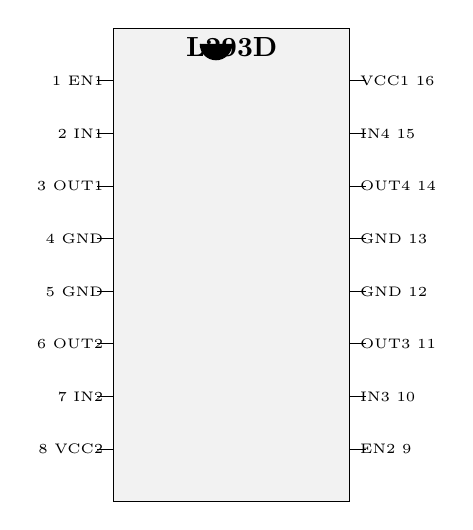
\begin{tikzpicture}[
    pin/.style={draw, rectangle, minimum width=0.6cm, minimum height=0.4cm, font=\tiny},
    ic/.style={draw, rectangle, minimum width=3cm, minimum height=6cm, fill=black!5}
]
    \node [ic] (l293d) {};
    \node [anchor=north, font=\bfseries] at (l293d.north) {L293D};
    \draw [fill=black] (l293d.north) ++(0,-0.2) arc (0:-180:0.2); 
    
    % Pins
    \foreach \i/\label in {1/EN1, 2/IN1, 3/OUT1, 4/GND, 5/GND, 6/OUT2, 7/IN2, 8/VCC2} {
         \node [left, font=\tiny] at ($(l293d.north west)!{\i/9}!(l293d.south west)$) {\i\ \label};
         \draw ($(l293d.north west)!{\i/9}!(l293d.south west)$) -- ++(-0.2,0);
    }
    \foreach \i/\label in {1/VCC1, 2/IN4, 3/OUT4, 4/GND, 5/GND, 6/OUT3, 7/IN3, 8/EN2} {
         \node [right, font=\tiny] at ($(l293d.north east)!{\i/9}!(l293d.south east)$) {\label\ \pgfmathparse{17-\i}\pgfmathprintnumber{\pgfmathresult}};
         \draw ($(l293d.north east)!{\i/9}!(l293d.south east)$) -- ++(0.2,0);
    }
\end{tikzpicture}
\end{answerdiagram}

\begin{itemize}
    \item \keyword{Dual H-Bridges}: Can control two DC motors independently
    \item \keyword{Heat Sink}: Ground pins provide heat dissipation
    \item \keyword{High Current}: Can drive up to 600mA per channel
    \item \keyword{Protection Diodes}: Internal flyback diodes for inductive loads
\end{itemize}
\end{solutionbox}

\begin{mnemonicbox}
\mnemonic{Enable, Input, Output, Power}
\end{mnemonicbox}

\questionmarks{5(b)}{4}{Draw and explain ADMUX register.}

\begin{solutionbox}
\textbf{ADMUX (ADC Multiplexer Selection Register) controls analog channel selection and result format in ATmega32.}

\begin{answerdiagram}{ADMUX Register}
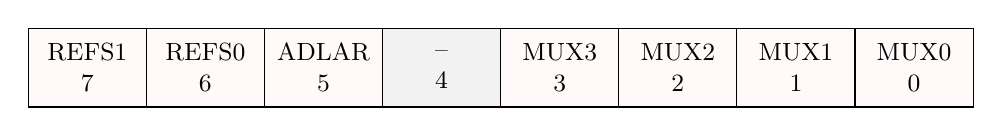
\begin{tikzpicture}[
    node distance=0cm,
    outer sep=0pt,
    bit/.style={draw, rectangle, minimum width=1.5cm, minimum height=1cm, align=center, font=\small}
]
    \node [bit, fill=pink!10] (b7) {REFS1\\7};
    \node [bit, fill=pink!10, right=of b7] (b6) {REFS0\\6};
    \node [bit, fill=pink!10, right=of b6] (b5) {ADLAR\\5};
    \node [bit, fill=gray!10, right=of b5] (b4) {--\\4};
    \node [bit, fill=pink!10, right=of b4] (b3) {MUX3\\3};
    \node [bit, fill=pink!10, right=of b3] (b2) {MUX2\\2};
    \node [bit, fill=pink!10, right=of b2] (b1) {MUX1\\1};
    \node [bit, fill=pink!10, right=of b1] (b0) {MUX0\\0};
\end{tikzpicture}
\end{answerdiagram}

\begin{answertable}{ADMUX Bit Functions}
\begin{tabulary}{\linewidth}{|L|L|L|}
\hline
\textbf{Bits} & \textbf{Name} & \textbf{Function} \\ \hline
7:6 & REFS1:0 & Reference voltage selection \\ \hline
5 & ADLAR & ADC Left Adjust Result \\ \hline
3:0 & MUX3:0 & Analog channel selection \\ \hline
\end{tabulary}
\end{answertable}

\begin{itemize}
    \item \keyword{REFS1:0 Settings}: 00=AREF, 01=AVCC, 11=Internal 2.56V
    \item \keyword{Channel Selection}: MUX3:0 selects which ADC input to connect
    \item \keyword{Result Alignment}: ADLAR=1 shifts result left
\end{itemize}
\end{solutionbox}

\begin{mnemonicbox}
\mnemonic{Reference, Alignment, Multiplexer}
\end{mnemonicbox}

\questionmarks{5(c)}{7}{Explain Smart Irrigation System.}

\begin{solutionbox}
\textbf{A Smart Irrigation System uses embedded technology to efficiently manage water for plant cultivation based on environmental conditions.}

\begin{answerdiagram}{Smart Irrigation System Flowchart}
\begin{tikzpicture}[node distance=2cm, auto, >=latex, thick]
    \node [gtu block] (mcu) {Microcontroller\\(ATmega32)};
    
    % Inputs
    \node [gtu block, above left=of mcu] (soil) {Soil Moisture\\Sensors};
    \node [gtu block, left=of mcu] (temp) {Temp/Humidity\\Sensors};
    \node [gtu block, below left=of mcu] (level) {Water Level\\Sensors};
    \node [gtu block, above=of mcu] (forecast) {Weather\\Forecast};
    
    % Outputs
    \node [gtu block, above right=of mcu] (pump) {Water Pump\\Control};
    \node [gtu block, right=of mcu] (valve) {Valve\\Control};
    \node [gtu block, below right=of mcu] (ui) {User\\Interface};
    
    % Connections
    \draw [->] (soil) -- (mcu);
    \draw [->] (temp) -- (mcu);
    \draw [->] (level) -- (mcu);
    \draw [->] (forecast) -- (mcu);
    
    \draw [->] (mcu) -- (pump);
    \draw [->] (mcu) -- (valve);
    \draw [->] (mcu) -- (ui);
\end{tikzpicture}
\end{answerdiagram}

\begin{answertable}{Smart Irrigation Components}
\begin{tabulary}{\linewidth}{|L|L|}
\hline
\textbf{Component} & \textbf{Function} \\ \hline
Soil Moisture Sensors & Measure water content in soil \\ \hline
Temperature/Humidity & Monitor environmental conditions \\ \hline
Valves & Control water flow to different zones \\ \hline
Pump Control & Activate water pumps when needed \\ \hline
Microcontroller & Process sensor data and control outputs \\ \hline
User Interface & Allow monitoring and manual control \\ \hline
\end{tabulary}
\end{answertable}

\textbf{Key Features:}
\begin{itemize}
    \item \keyword{Automated Watering}: Waters plants only when soil moisture falls below threshold
    \item \keyword{Weather Adaptation}: Adjusts watering schedule based on forecast
    \item \keyword{Zone Control}: Individual watering schedules for different areas
    \item \keyword{Water Conservation}: Uses minimum necessary water
\end{itemize}
\end{solutionbox}

\begin{mnemonicbox}
\mnemonic{Sense, Decide, Conserve, Grow}
\end{mnemonicbox}

\questionmarks{5(a OR)}{3}{Draw circuit diagram to interface DC motor with ATmega32 using L293D motor driver.}

\begin{solutionbox}
\textbf{The circuit connects a DC motor to ATmega32 through L293D for bidirectional control.}

\begin{answerdiagram}{DC Motor Interfacing}
\begin{tikzpicture}[auto, >=latex, thick, node distance=2.5cm]
    \node [gtu block] (mcu) {ATmega32};
    \node [gtu block, right=of mcu] (driver) {L293D};
    \node [draw, circle, right=of driver, minimum size=1.5cm] (motor) {M};
    
    % Connections
    \draw [->] ([yshift=0.5cm]mcu.east) -- node[above, font=\tiny] {PB0} ([yshift=0.5cm]driver.west) node[left, font=\tiny] {IN1};
    \draw [->] (mcu.east) -- node[above, font=\tiny] {PB1} (driver.west) node[left, font=\tiny] {IN2};
    \draw [->] ([yshift=-0.5cm]mcu.east) -- node[above, font=\tiny] {PB2} ([yshift=-0.5cm]driver.west) node[left, font=\tiny] {EN1};
    
    \draw [->] ([yshift=0.5cm]driver.east) -- ([yshift=0.5cm]motor.west);
    \draw [->] ([yshift=-0.5cm]driver.east) -- ([yshift=-0.5cm]motor.west);
    
    % Power
    \draw (driver.north) -- ++(0,0.5) node[above] {VCC2 (12V)};
\end{tikzpicture}
\end{answerdiagram}

\textbf{Control Logic:}
\begin{answertable}{Motor Control Logic}
\begin{tabulary}{\linewidth}{|C|C|C|L|}
\hline
\textbf{IN1} & \textbf{IN2} & \textbf{EN1} & \textbf{Status} \\ \hline
0 & 0 & 1 & Stop \\ \hline
1 & 0 & 1 & Clockwise \\ \hline
0 & 1 & 1 & Counter-Clockwise \\ \hline
1 & 1 & 1 & Stop \\ \hline
\end{tabulary}
\end{answertable}
\end{solutionbox}

\begin{mnemonicbox}
\mnemonic{Enable and Direction Control Motor}
\end{mnemonicbox}

\questionmarks{5(b OR)}{4}{Draw and Explain I2C based device interfacing diagram with ATmega32.}

\begin{solutionbox}
\textbf{I2C (Inter-Integrated Circuit) is a two-wire serial bus for connecting multiple devices to a microcontroller.}

\begin{answerdiagram}{I2C Interfacing}
\begin{tikzpicture}[auto, >=latex, thick]
    % Bus Lines
    \draw [thick] (0,4) node[left]{SDA} -- (10,4);
    \draw [thick] (0,2) node[left]{SCL} -- (10,2);
    
    % Pull-ups
    \draw (2,4) -- (2,5) to[R, l=4.7k] (2,6) node[above]{VCC};
    \draw (8,2) -- (8,5) to[R, l=4.7k] (8,6) node[above]{VCC};
    
    % Devices
    \node [gtu block] (mcu) at (1,0) {ATmega32\\(Master)};
    \node [gtu block] (dev1) at (5,0) {Device 1\\(EEPROM)};
    \node [gtu block] (dev2) at (9,0) {Device 2\\(Sensor)};
    
    % Connections
    \draw (mcu.north) ++(-0.5,0) -- ++(0,4); % SDA
    \draw (mcu.north) ++(0.5,0) -- ++(0,2);  % SCL
    \fill (0.5, 4) circle (2pt);
    \fill (1.5, 2) circle (2pt);
    
    \draw (dev1.north) ++(-0.5,0) -- ++(0,4);
    \draw (dev1.north) ++(0.5,0) -- ++(0,2);
    \fill (4.5, 4) circle (2pt);
    \fill (5.5, 2) circle (2pt);
    
    \draw (dev2.north) ++(-0.5,0) -- ++(0,4);
    \draw (dev2.north) ++(0.5,0) -- ++(0,2);
    \fill (8.5, 4) circle (2pt);
    \fill (9.5, 2) circle (2pt);
\end{tikzpicture}
\end{answerdiagram}

\begin{itemize}
    \item \keyword{SDA}: Serial Data Line (Bidirectional)
    \item \keyword{SCL}: Serial Clock Line (Master generated)
    \item \keyword{Pull-up Resistors}: Required on both lines
\end{itemize}
\end{solutionbox}

\begin{mnemonicbox}
\mnemonic{Start, Address, Acknowledge, Data, Stop}
\end{mnemonicbox}

\questionmarks{5(c OR)}{7}{Explain IoT based Home Automation System.}

\begin{solutionbox}
\textbf{An IoT-based Home Automation System connects household devices to the internet for remote monitoring and control.}

\begin{answerdiagram}{IoT Home Automation Architecture}
\begin{tikzpicture}[node distance=2cm, auto, >=latex, thick]
    \node [gtu block] (cloud) {Cloud Services};
    \node [gtu block, below=of cloud] (gateway) {Internet Gateway};
    \node [gtu block, below=of gateway] (controller) {Home Controller\\(ATmega32/ESP32)};
    
    % End devices
    \node [gtu block, below left=of controller] (lights) {Light/HVAC};
    \node [gtu block, below right=of controller] (security) {Security};
    \node [gtu block, right=of controller] (sensors) {Sensors};
    
    % User Interfaces
    \node [gtu block, left=of gateway] (app) {Mobile App};
    
    % Connections
    \draw [<->] (cloud) -- (gateway);
    \draw [<->] (gateway) -- (controller);
    \draw [<->] (controller) -- (lights);
    \draw [<->] (controller) -- (security);
    \draw [<-] (controller) -- (sensors);
    \draw [<->] (gateway) -- (app);
\end{tikzpicture}
\end{answerdiagram}

\begin{answertable}{Home Automation Components}
\begin{tabulary}{\linewidth}{|L|L|}
\hline
\textbf{Component} & \textbf{Function} \\ \hline
Controller & Central processing unit \\ \hline
Sensors & Monitor environmental conditions \\ \hline
Actuators & Control lights, appliances, locks \\ \hline
Gateway & Connects local devices to internet \\ \hline
User Interface & App, voice control, dashboard \\ \hline
Cloud Services & Storage, processing, remote access \\ \hline
\end{tabulary}
\end{answertable}

\begin{itemize}
    \item \keyword{Remote Access}: Control from anywhere
    \item \keyword{Voice Control}: Integration with assistants
    \item \keyword{Energy Management}: Optimize consumption
    \item \keyword{Automation}: Scheduling and scene setting
\end{itemize}
\end{solutionbox}

\begin{mnemonicbox}
\mnemonic{Connect, Control, Monitor, Automate, Learn}
\end{mnemonicbox}

\end{document}





